
%%
%%  Beam Loading Paper '17
%% ***************************
%%  Veronica K. Berglyd Olsen
%%

\documentclass[aps,prstab,reprint,amsmath,amssymb,groupedaddress]{revtex4-1}
\bibliographystyle{apsrev4-1}

\usepackage{hyperref}
\hypersetup{colorlinks=true, citecolor=blue, urlcolor=blue, linkcolor=blue}

\usepackage{graphicx}


% Custom Commands
%*****************

% Text
%~ \newcommand{\eq}[1]{Eq. \ref{#1}}
%~ \newcommand{\fig}[1]{Fig. \ref{#1}}
%~ \newcommand{\tbl}[1]{Table \ref{#1}}

% Math
\newcommand{\unit}[1]{\,\mathrm{#1}}
\newcommand{\funit}[2]{\,\mathrm{#1}/\mathrm{#2}}
\newcommand{\mexp}[1]{\mathrm{e}{#1}}
\newcommand{\nexp}[1]{\times 10^{#1}}

% ******************************************************************************************************************** %
\begin{document}
% ******************************************************************************************************************** %

%~ Eric's Comments
%~ Sec N: Beam loading [in this section we describe the interesting physics, based on a single parameters set]
%~ - describe proton beam wake structure [similar to that of a modulated proton beam] (simulation results to show:
%~   unloaded wake)
%~ - by varying the current of the electron beam, the electron beam may load the wake and the longitudinal field can be
%~   flatten and energy spread reduced [well known result, Tzoufras] 
%~ - the electron beam blows out the remaining plasma electrons. The transverse fields are dominated by the linear
%~   focusing fields originating from the ion background, leading to emittance preservation of the part of the electron
%~   beam inside the bubble [loading of a quasi-linear wake, and still get emittance preservation: this is new]
%~   (simulation results to show: loaded wake, with bubble - many different aspects of this, trans., long. field,
%~   electron densities etc. )
%~ - the acceleration and the transverse emittance stable on long timescales (simulation results to show: transverse and
%~   longitudinal phase spaces, space long simulation)
%~ - in this regime, emittance preservation is robustness to drive-witness offset [this is new] (simulation results to
%~   show: transverse and longitudinal phase spaces, long offset simulation)
%~ Sec N+1: Parameter optimization, or, parameter scaling [in this section we describe how to optimize the electron
%~ beam, and preferably some scalings]
%~ - how to select electron beam parameters:
%~ - longitudinal parameters bunch length and current (simulations results to show: overloaded/underloaded cases)
%~ - transverse parameters of electron emittance / matching [too large, outside bubble.  Do we see increased head
%~   erosion -> faster decay]?  (simulations results to show: evolution of high emittance vs low emittance cases)
%~ (- plasma density?)


%~ Patric's Comments
%~ - Self-modulation as a driver
%~ - SM does not reach blow out
%~ - SM does not preserve emittance and produces large energy spread and parameters may evolve along the accelerator,
%~   not desirable
%~ - Beam loading for narrow energy spread
%~ - Beam loading in linear regime (old papers from SLAC in the 80's, then Katsouleas for PWFA) and nonlinear regime
%~   (Tzoufras) well know
%~ - Propose "new regime" in the SM case, beam loading and blowout to get emittance preservation
%~ - Limitation as for PWFA driver, must use some of the W bunch to reach the blowout, it is kind of like the early SLAC
%~   experiments (84GeV) where the W-bunch is like the D-bunch in these experiments, but in a plasma prepared by the p+
%~   bunch and the SM
%~ - maybe also something about the fact that 200pC in a 60µm bunch corresponds to a 1kA current, much larger than the
%~   p+ bunch current, because of the fact that the wakefields are driven my multiple bunches?
%~ As for N+2, I am a firm supporter of on-axis injection ... and most of the issue with that has to do with the plasma
%~ ramp, otherwise it would be a non-issue (assuming of course that one can split the plasma in two sections). It is in
%~ itself a topic of research, so I think we can only state a few things ...


\title{Emittance preservation of an electron beam in a loaded quasi-linear plasma wakefield}

\author{Veronica K. Berglyd Olsen}
\email[]{v.k.b.olsen@cern.ch}

\author{Erik Adli}
\affiliation{University of Oslo, Oslo, Norway}

\author{Patric Muggli}
\affiliation{Max Planck Institute for Physics, Munich, Germany}
\affiliation{CERN, Geneva, Switzerland}

\date{\today}

\begin{abstract}
We investigate beam loading and emittance preservation for a high-charge electron beam being accelerated in quasi-linear
plasma wakefield driven by a short proton beam. The structure of the wakefield is similar to that of a long, modulated
proton beam, such as the one being studied by AWAKE.  We show that by exploiting two well known effects, full blow out
of plasma electrons by the accelerated beam, and beam loading of the wake field, the electron beam can be accelerated
without significant emittance growth.
\end{abstract}

\maketitle

% ******************************************************************************************************************** %
\section{Introduction}\label{S:I}
% interested from SMI/AWAKE
% requirements for AWAKE Run 2
% ******************************************************************************************************************** %

Beam driven plasma wakefield accelerators have the potential to offer compact linear accelerators with high energy
gradients, and have been of interest for several decades \cite{chen:1985}. With a relativistic charged particle drive
beam travelling through a plasma, a strong wakefield is excited, that can be loaded by a trailing witness beam. When the
witness beam optimally loads the wakefield, an increase in absolute energy spread can be kept to a minimum. The concept
has been demonstrated experimentally in the past using electron drive beams accelerating electron witness beams
\cite{rosenzweig:1988, blumenfeld:2007, kallos:2008}. AWAKE at CERN is a proof of concept beam driven plasma wakefield
accelerator experiment using a proton drive beam delivered by the SPS accelerator \cite{awake_collaboration:2014}.

A major challenge with plasma wakefield accelerators is, however, to accelerate a beam while keeping energy spread and
emittance growth to a minimum. In the well described linear case where the beam density $n_{b}$ is much smaller than the
plasma density $n_{0}$, a non-linear transverse focusing force causes emittance growth of the witness beam. the beam
will also see a transversely and longitudinally varying accelerating field causing a spread in energy after the beam has
been accelerated \cite{katsouleas:1987}. In the non-linear regime, where $n_{b} > n_{0}$, a bubble is formed by the
transverse oscillations of the plasma electrons, forming a sheet around an evacuated area filled with only ions. The
ions, assumed stationary, form an uniform density ion channel creating a focusing force that varies linearly with
radius. This produces a focusing force that preserves emittance \cite{lu:2006-1, lu:2006}.

In this paper we present simulation results showing how we can use the non-linear wakefields driven by the head of a
high charge density witness beam to reduce energy spread and emittance growth in the rest of the beam, while being
accelerated by a proton drive beam producing quasi-linear wakefields.

% ******************************************************************************************************************** %
\subsection[\label{S:I:SMI}]{Self-modulation as a Driver}
%~ Patric's Comments
%~ - Self-modulation as a driver
%~ - SM does not reach blow out
%~ - SM does not preserve emittance and produces large energy spread and parameters may evolve along the accelerator,
%~   not desirable
% ******************************************************************************************************************** %

A train of electron drive bunches with a separation $\lambda_{pe}$ and a length $l_{b} \ll \lambda_{pe}$, where the
plasma wavelength $\lambda_{pe} = 2\pi c/\omega_{pe}$ and the plasma frequency $\omega_{pe} = (n_{0} e^{2} / m_{e}
\epsilon_{0})^{1/2}$, produces a field $E_{z}$ that increases for each drive bunch \cite{chen:1985}. A tailing witness
beam loading the peak accelerating phase of this field will gain energy from the wakefield from all of the drive bunches
when they are properly phased with respect to the wakefields. Acceleration of an electron witness beam driven by two
electron drive beams has been demonstrated at Brookhaven National Laboratory \cite{muggli:2011}.

The energy carried by electron drive bunches used in previous experiments were typically small -- on the order of
$100\unit{J}$ -- and the propagation length typically $<1\unit{m}$ \cite{blumenfeld:2007,caldwell:2009}. Higher energy
electron beam can be improve the propagation length and thus the energy of the accelerated beam. For instance, the
energy of a high-charge electron beam accelerated to $1\unit{TeV}$, similar to the beam that could be produced by the
international linear collider with $1\nexp{10}$ electrons, is $1.6\unit{kJ}$. By using electron beams or lasers pulses
as drivers, a large number of plasma stages is required. However, staging plasma accelerators without reducing the
effective gradient and spoiling the beam quality is challenging \cite{steinke:2016,lindstrom:2016}.

Proton beams available at CERN carry significantly more energy, $19\unit{kJ}$ for the SPS beam \cite{gschwendtner:2016},
allowing for much longer plasma wakefield accelerator stages. The SPS beam is, unfortunately, orders of magnitude longer
than the plasma wavelengths needed for such applications. This can be resolved by letting the proton beam undergo
self-modulation before injecting the witness beam into accelerating structure. The self-modulation of the beam is
produced by the transverse fields generated by the beam acting upon itself, causing regions of the beam to rapidly
defocus \cite{kumar:2010}. The modulation frequency is close to that of the plasma, and produces a train of short proton
bunches along the beam axis with a surrounding halo of defocused particles. This train of bunches resonantly produces
wakefields to larger amplitudes.

% ******************************************************************************************************************** %
\subsection{AWAKE Run 2}\label{S:I:AWAKE}
% ******************************************************************************************************************** %

The AWAKE experiment, currently in its first stages of operation at CERN, uses a $400\unit{GeV}$ beam delivered by the
SPS as its driver, and a single $10\unit{m}$ plasma stage with a nominal plasma density of $7\nexp{14}\unit{cm}^{-3}$
\cite{gschwendtner:2016}. This plasma density corresponds to $\lambda_{pe} = 1.26\unit{mm}$ -- matched to the transverse
size of the SPS proton beam such that $k_{pe}\sigma_{x,y} = 1$, where $k_{pe} = 2\pi/\lambda_{pe}$ is the plasma wave
number.

The aim of the first phase of Run 1 of the experiment is to demonstrate self-modulation of the proton beam. The aim of
the second phase in 2018 is to sample the wakefield with a long electron beam $\simeq\lambda_{pe}$. The study presented
here is for Run 2 \cite{adli:2016}, which aims to demonstrate acceleration of a short electron beam, $\ll\lambda_{pe}$,
to high energy with a minimal increase in emittance and absolute energy spread.

\begin{figure}[hbt]
    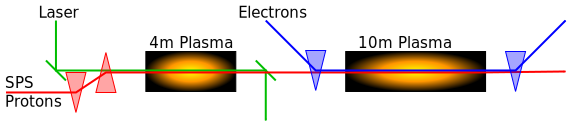
\includegraphics[width=0.99\linewidth,trim={1mm 2mm 1mm 2mm},clip]{figures/figAWAKE}
    \caption{\label{Fig:AWAKER2} A simplified illustration of the experimental setup for AWAKE Run 2. The SPS proton
        beam undergoes self-modulation in the first plasma section. The electron witness beam is injected into the
        accelerating structure, and undergoes acceleration in the second plasma stage
        \cite{berglyd_olsen:2015, adli:2016}.}
\end{figure}

The plans for AWAKE Run 2 proposes to use two plasma sections, illustrated in figure \ref{Fig:AWAKER2}. The first
section of $4\unit{m}$ is the self-modulation stage where the proton beam undergoes self-modulation without the electron
beam present. The electron witness beam is then injected into the modulated proton beam before stage two, where it
undergoes acceleration.

Using the SPS proton beam as driver, the self-modulated proton beam does not produce a full non-linear wakefield, and
not all plasma electrons are therefore evacuated from the plasma bubble. The result is that the focusing force does not
increase linearly with radius. The small size of the accelerating structure produced by the self-modulated beam also
puts constraints on the size of the electron witness beam, and thus its charge and current, if at the same time we wish
to prevent large energy spread. By matching the transverse size of the beam at a given emittance to the plasma density,
we prevent large amplitude oscillations which may cause additional energy spread as well as emittance growth.

%~ Eric's version:
%~ The key idea in this paper is that while the proton beam wake is not fully blown-out, and thus leading to non-linear
%~ focusing forces, the electron beam, if intense enough, may load the field and at the same time create its own ion
%~ bubble. As will be shown, exploiting these two well known effects, the electron beam can be accelerated for long
%~ distances without significant emittance growth.

%~ Patric's version:
The key idea is to have enough charge in the witness beam to at the same time load the wakefield to produce low
relative energy spread $\Delta E/E$, and blow out the electrons left in the accelerating structure to reach conditions
that preserves emittance.

% ******************************************************************************************************************** %
\section[\label{S:M}]{Method}
%- explain analogy of short-bunch, SMI case, by referring to earlier Veronica-papers
%- simulation setup PIC/quickpic OS
% ******************************************************************************************************************** %

A main focus of this study is on the loading of the wakefields driven by the proton beam. In order to eliminate other
factors that may affect this, like decay and defocusing of the proton beam, we tried several approaches to create a
stable drive beam structure based in previous self-modulation studies.

In these studies we used a short, pre-modulated proton beam with similar structure to the beam produced by the
self-modulation of the SPS beam in AWAKE. These studies were done using the full PIC code Osiris \cite{fonseca:2002}
using 2D cylindrical-symmetric simulations and primarily looked at beam loading, energy gain and energy spread
\cite{berglyd_olsen:2015, berglyd_olsen:2016}.

In order to study the witness beam emittance evolution we turned to the recently released open source version of
QuickPIC. QuickPIC is a fully relativistic 3D quasi-static PIC code \cite{huang:2006, an:2013}. It does not suffer from
the numerical Cherenkov effect that full PIC codes do \cite{godfrey:1974,lehe:2013}, making it a well suited tool to
study emittance preservation.

%~ In order to evaluate the quality of the accelerated bunch it was also necessary to study emittance evolution. However,
%~ full PIC codes are vulnerable to numerical growth of emittance caused by the ``numerical Cherenkov effect''
%~ \cite{godfrey:1974}. This is a know issue with the Yee EMF solver which causes the phase velocity of electromagnetic
%~ fields to be lower than $c$ while the beam moves very close to $c$. The effect can be mitigated somewhat by replacing
%~ the Yee solver with a solver designed by Lehe \cite{lehe:2013}. Our simulations showed that this numerical effect is
%~ still prominent in the high density regions of our very compact electron bunch, making it difficult to distinguish
%~ emittance growth from the physics from that originating from numerical error.

\begin{figure}[hbt]
    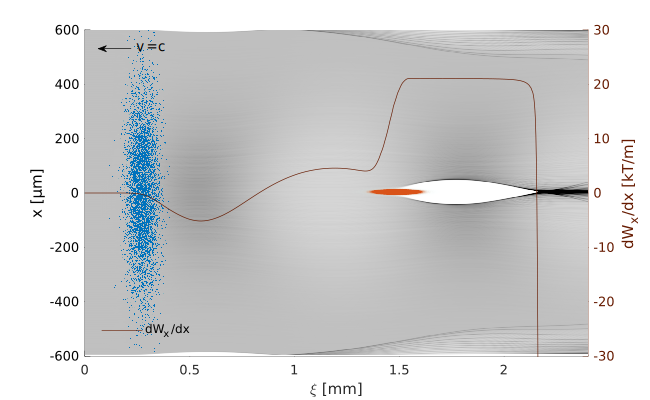
\includegraphics[width=\linewidth,trim={2mm 0mm 2mm 0mm},clip]{figures/plasmaDenTWake}
    \caption{\label{Fig:PlasmaDenTWake} The plasma density in grey with the drive beam (blue) and the witness beam (red)
        superimposed. The line plot indicates the transverse wakefield gradient $dW_{x}/dx$ where
        $W_{x} = E_{x} - v_{b} B_{y}$, evaluated along the beam axis.}
\end{figure}

% ******************************************************************************************************************** %
\subsection{Drive Beam Parameters}\label{S:M:Setup}
%~ Patric's Comments
%~ - Self-modulation as a driver
%~ - SM does not reach blow out
%~ - SM does not preserve emittance and produces large energy spread and parameters may evolve along the accelerator,
%~   not desirable
% ******************************************************************************************************************** %

%~ In these simulations we use a single proton drive beam that sets up a wakefield comparable to that which we expect to
%~ see from the self-modulated SPS beam in the second plasma cell of AWAKE Run 2 (Figure \ref{Fig:AWAKER2}).

The baseline AWAKE drive beam current is insufficient to reach the non-linear regime and produce a plasma bubble. When
the SPS beam, containing $3\nexp{11}$ protons \cite{gschwendtner:2016}, enters the second plasma stage, the peak
electric field is expected to be $500-600\funit{MV}{m}$. The plasma electrons are only depleted to around $65\%$ of
nominal plasma density at the point where we inject the electron beam \cite{awake_collaboration:2016}. In our simulation
these conditions are replicated using a single proton beam of $1.46\nexp{10}$ protons, or $2.34\unit{nC}$ and
$7\unit{kA}$.

The peak density of the simulation drive beam is $0.83\cdot n_{0}$, producing a quasi-linear wakefield. The single bunch
setup uses the baseline proton beam energy of $400\unit{GeV}$ and transverse size $\sigma_{x} = 200\unit{\mu m}$. We
also set the length of the drive beam to $\sigma_{z} = 40\unit{\mu m}$. We are not considering the evolution of the
proton beam itself in this study, so in order to create a stable environment to study the evolution of the witness beam
we prevent the proton beam from evolving radially by increasing the particle mass by 6 orders of magnitude.

% ******************************************************************************************************************** %
\subsection{Witness Beam Parameters}\label{S:M:Setup}
% ******************************************************************************************************************** %

Beam loading of a short witness beam is sensitive to its position relative to the electric field \cite{tzoufras:2009}.
A low gamma witness beam can easily drift out of phase with the drive beam wakefield. The drift of the beams is
proportional to $\gamma^{-2}$, so to eliminate initial de-phasing of the witness beam, initial beam energy was set such
that $\gamma_{eb} = \gamma_{pb} = 426.3$, giving an energy of $217\unit{MeV}$. A lower initial value is likely to be
sufficient \cite{berglyd_olsen:2015}.

In these simulations we have used a matched beam for an initial normalised emittance of $\epsilon_{N} = 2\unit{\mu m}$.
The beam matching relation is given by
\begin{equation}
    \beta = \frac{\sigma_{x,y}^{2}\gamma}{\epsilon_{N}}
          = \frac{c}{\omega_{pe}}\sqrt{2\gamma}, \label{EQ:MatchedB}
    % = c\sqrt{\frac{m_{e}\varepsilon_{0}}{n_{pe}e^{2}}2\gamma}
\end{equation}
where $\beta$ is the Twiss parameter. It then follows that the transverse profile of the beam must satisfy
\begin{equation}
    \sigma_{x,y}^{2} = c\epsilon_{N}\sqrt{2\frac{m_{e}\varepsilon_{0}}{n_{pe}e^{2}\gamma}} \label{EQ:MatchedR}
\end{equation}
in order to be matched to a given plasma density, initial emittance and energy. This relation requires a very narrow
beam with a $\sigma_{x,y}$ of $5.25\unit{\mu m}$ compared to the drive beam $\sigma_{x,y} = 200\unit{\mu m}$. The charge
density of this compact witness beam reaches that of the plasma density at only a few $\unit{pC}$, but reaches optimal
beam loading at around $100-200\unit{pC}$. The implication here being that the witness beam produces its own non-linear
wakefield already at the head of the beam. The majority of the electrons within it will therefore see a linear focusing
force preventing the bulk of the beam from undergoing emittance growth.

The relatively small size of the witness beam compared to the proton beam put some restrictions on the transverse
resolution of the witness beam as we need a simulation box wide enough to contain the larger beam while resolving the
narrower one (see figure \ref{Fig:PlasmaDenTWake}). We used a transverse grid cell size of $1.17\unit{\mu m}$, and of
$2.34\unit{\mu m}$ for the longitudinal grid cells for the simulations presented in section \ref{S:BL}. The witness beam
was simulated with $16.8\nexp{6}$ non-weighted particles. The witness beam has a total charge of $100\unit{pC}$, a
$\sigma_{z}=60\unit{\mu m}$, and a $\sigma_{x}=5.25\unit{\mu m}$ matching an initial normalised emittance
$\epsilon_{0} = 2\unit{\mu m}$. We refer to this parameter set as our base case.

\begin{figure}[hbt]
    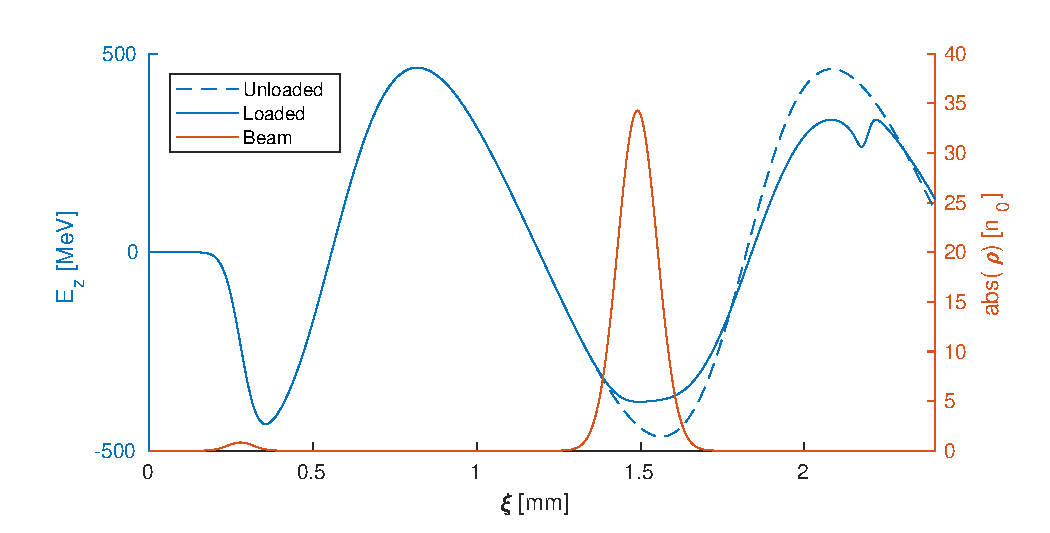
\includegraphics[width=\linewidth,trim={2mm 0mm 2mm 0mm},clip]{figures/beamLoading}
    \caption{\label{Fig:BeamLoading} The top plot shows the unloaded longitudinal electric field with no witness beam
        (dashed blue line) and the loaded field (whole blue line) along the beam axis. The beam density along the axis
        for both beams are shown in red. The bottom plot compares the plasma densities along the beam axis for a drive
        beam with no witness beam (dashed green line), witness beam with no drive beam (dash-dotted green line), and
        both beams present (whole green line). $\xi = z - tc$ is the position in the simulation box, moving towards the
        left.}
\end{figure}

\begin{figure}[hbt]
    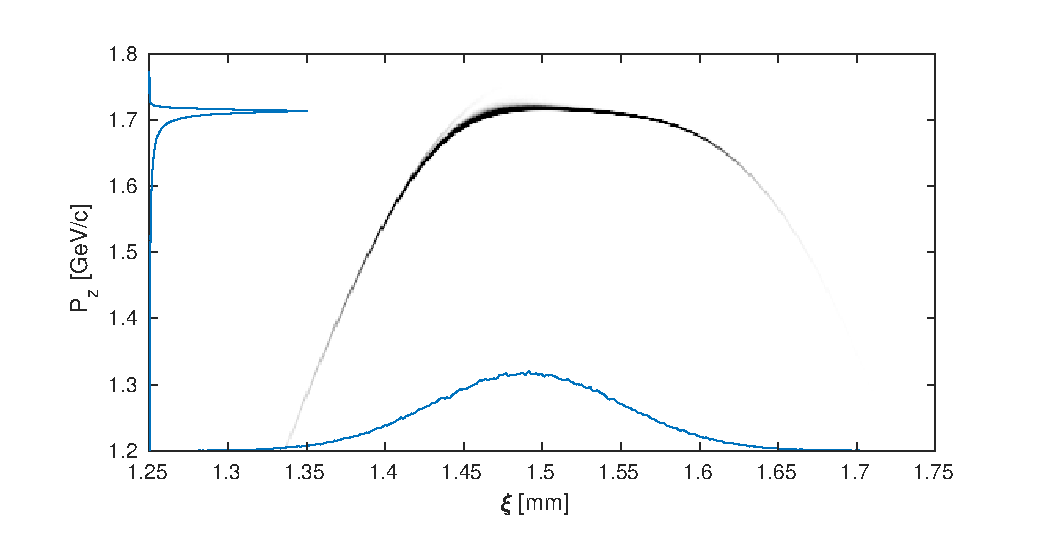
\includegraphics[width=\linewidth,trim={2mm 0mm 2mm 0mm},clip]{figures/beamPhaseSpace}
    \caption{\label{Fig:BeamPS} The phase space charge distribution of a $100\unit{pC}$, $60\unit{\mu m}$ long witness
        beam after $4\unit{m}$ of plasma. The mean momentum is $1.67\unit{GeV/c}$ with an RMS energy spread of
        $87\unit{MeV/c}$ ($5.2\%$) for the full beam.}
\end{figure}

\begin{figure*}[hbt]
    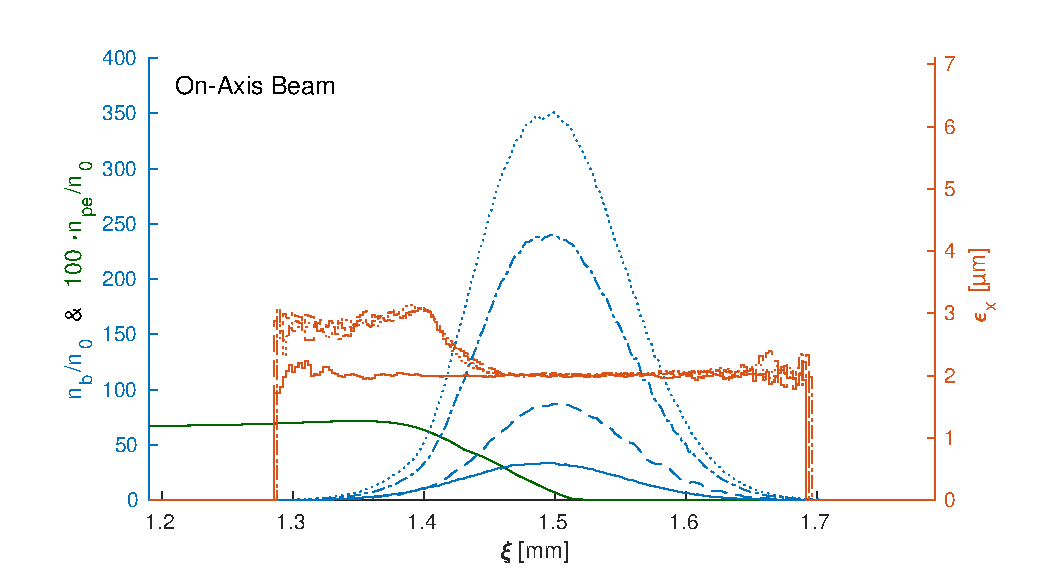
\includegraphics[width=0.495\linewidth,trim={2mm 0mm 2mm 0mm},clip]{figures/beamEmittance}
    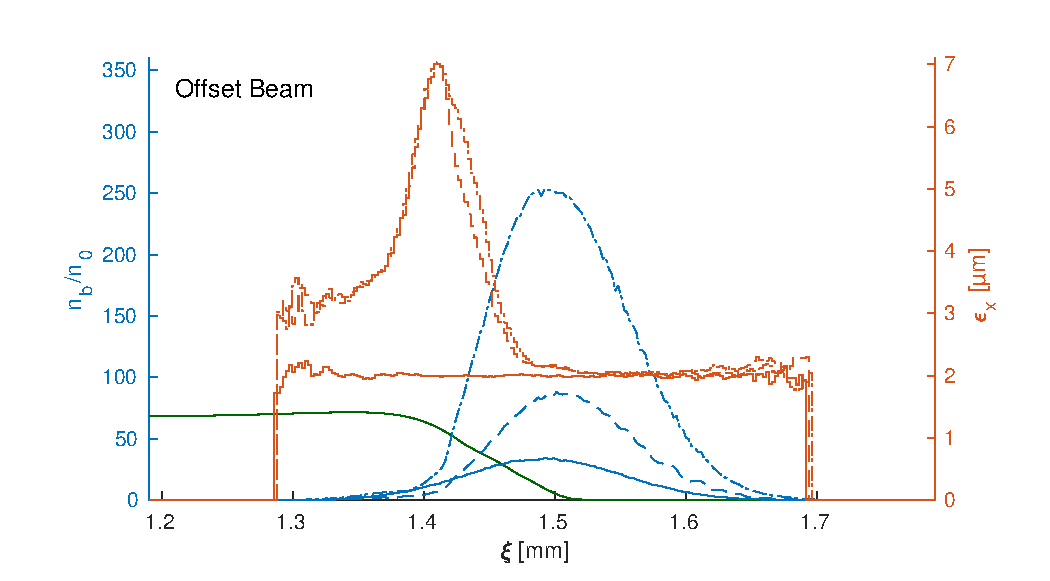
\includegraphics[width=0.495\linewidth,trim={2mm 0mm 2mm 0mm},clip]{figures/beamEmittanceOffset}
    \caption{\label{Fig:BeamEmitt} Beam density in blue along the beam axis for an on-axis beam with respect to the
        drive beam axis (left), and an offset beam (right) with an offset of one $\sigma_{x} = 5.24\unit{\mu m}$ in the
        x-plane. At four different positions $z$ in the plasma stage. The red lines show a moving window calculation of
        transverse normalised emittance. The moving window calculation uses longitudinal slices of
        $l = 4\times\Delta\xi = 9.38\unit{\mu m}$ with a step of $\Delta\xi$. Only slices with more than $100$ macro
        particles have been included. The plasma density profile is included in green, and scaled up by a factor of
        $100$ to be visible. These simulations were run with an LHC energy drive beam of $7\unit{TeV}$}
\end{figure*}

\begin{figure*}[hbt]
    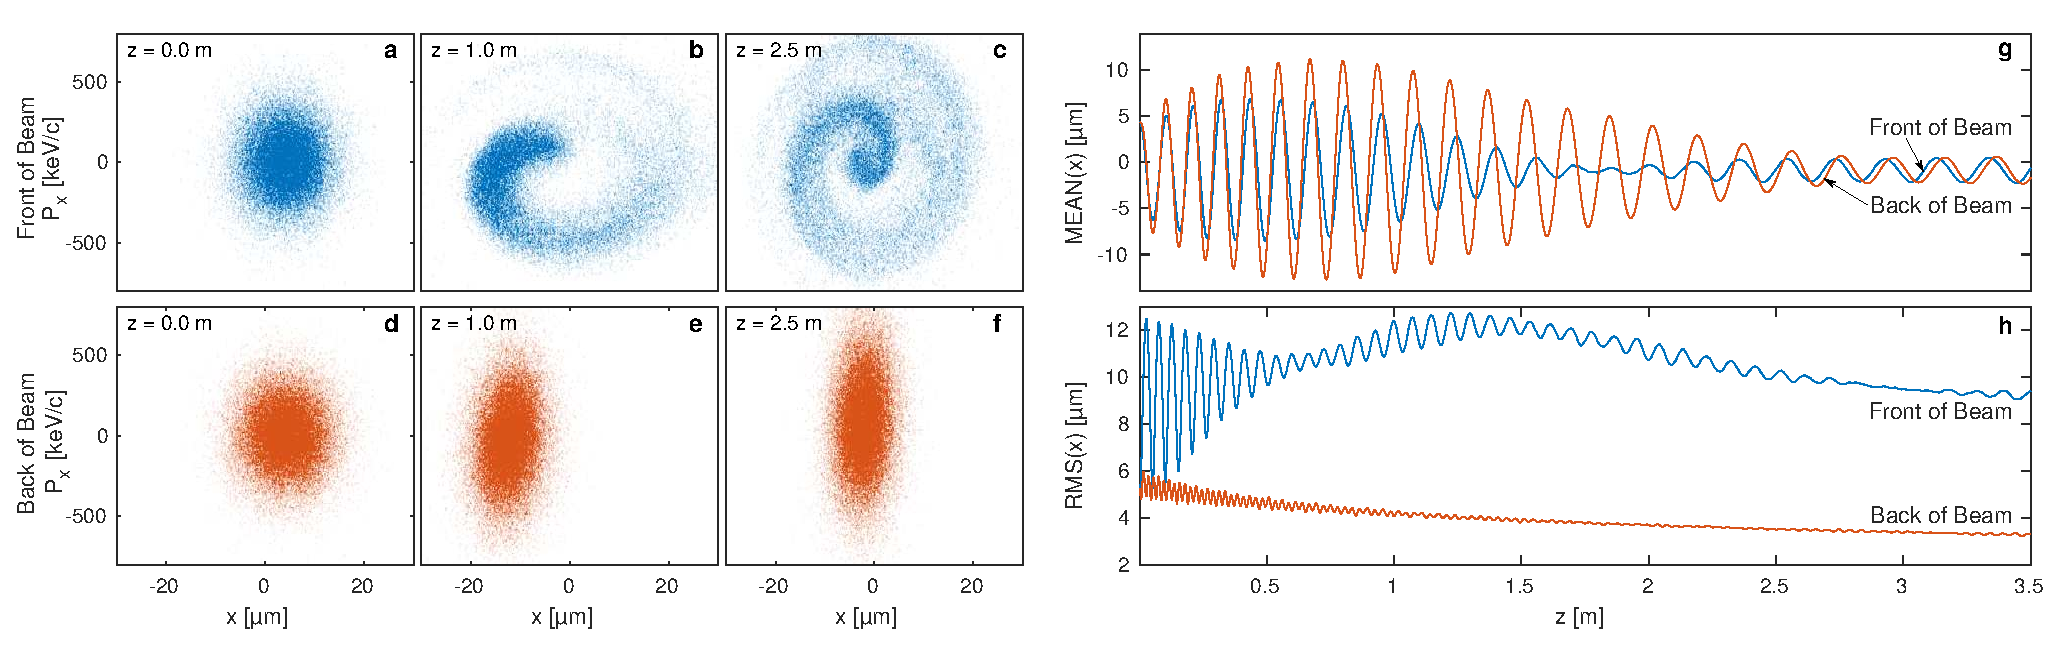
\includegraphics[width=\linewidth,trim={0mm 0mm 0mm 0mm},clip]{figures/beamFilamentationAll}
    \caption{\label{Fig:BeamFilament} Plots \textbf{a} to \textbf{f} show the transverse phase space of the offset
        electron beam at different plasma positions. Plot \textbf{g} shows the macro particle mean position, and plot
        \textbf{h} their RMS spread. Plots \textbf{a}, \textbf{b} and \textbf{c}, as well as the blue lines in plots
        \textbf{g} and \textbf{h} represent particles with position $1.40\unit{\mu m} < \xi < 1.42\unit{\mu m}$. Plots
        \textbf{d}, \textbf{e} and \textbf{f}, and the red lines in plots \textbf{g} and \textbf{h} represent particles
        with position $1.55\unit{\mu m} < \xi < 1.57\unit{\mu m}$.}
\end{figure*}

% ******************************************************************************************************************** %
\section{Beam Loading}\label{S:BL}
%~ Eric's Comments
%~ Sec N: Beam loading [in this section we describe the interesting physics, based on a single parameters set]
%~ - describe proton beam wake structure [similar to that of a modulated proton beam] (simulation results to show:
%~   unloaded wake)
%~ - by varying the current of the electron beam, the electron beam may load the wake and the longitudinal field can be
%~   flatten and energy spread reduced [well known result, Tzoufras]
%~ - the electron beam blows out the remaining plasma electrons. The transverse fields are dominated by the linear
%~   focusing fields originating from the ion background, leading to emittance preservation of the part of the electron
%~   beam inside the bubble [loading of a quasi-linear wake, and still get emittance preservation: this is new]
%~   (simulation results to show: loaded wake, with bubble - many different aspects of this, trans., long. field,
%~   electron densities etc. )
%~ - the acceleration and the transverse emittance stable on long timescales (simulation results to show: transverse and
%~   longitudinal phase spaces, space long simulation)
%~ - in this regime, emittance preservation is robustness to drive-witness offset [this is new] (simulation results to
%~   show: transverse and longitudinal phase spaces, long offset simulation)
%~
%~ Patric's Comments
%~ - Beam loading for narrow energy spread
%~ - Beam loading in linear regime (old papers from SLAC in the 80's, then Katsouleas for PWFA) and nonlinear regime
%~   (Tzoufras) well know
%~ - Propose "new regime" in the SM case, beam loading and blowout to get emittance preservation
%~ - Limitation as for PWFA driver, must use some of the W bunch to reach the blowout, it is kind of like the early SLAC
%~   experiments (84GeV) where the W-bunch is like the D-bunch in these experiments, but in a plasma prepared by the p+
%~   bunch and the SM
%~ - maybe also something about the fact that 200pC in a 60µm bunch corresponds to a 1kA current, much larger than the
%~   p+ bunch current, because of the fact that the wakefields are driven my multiple bunches?
% ******************************************************************************************************************** %

The single drive beam setup is designed to produce similar initial conditions for the witness beam as the self-modulated
case. However, since the drive beam is prevented from significant transverse evolution, we are presented with an
idealised case where the electron witness beam sees consistent wakefields throughout the plasma stage. The $E_{z}$-field
generated by the proton drive beam is seen as the blue line in figure \ref{Fig:BeamLoading}, shown with and without the
electron beam present. With a proton beam density $n_{pb} \simeq n_{0}$, we are in the quasi-linear regime
\cite{rosenzweig:2010}. The dashed green line in the lower part of figure \ref{Fig:BeamLoading} shows that the on-axis
plasma density has a depletion of $67\%$, close to what we see in full scale reference simulations for AWAKE Run 2
\cite{awake_collaboration:2016}.

%~ The witness beam generates its own wakefield, which in the accelerating phase partially cancels out the $E_{z}$ field
%~ generated by the drive beam. For a finite length beam this causes the particles in the tail of the witness beam to be
%~ accelerated less than those at the front resulting in higher energy spread in exchange for higher energy transfer
%~ \cite{van_der_meer:1985}. A beam profile $\rho_{b}(\xi)$ that perfectly flattens the
%~ accelerating field within the witness beam will reduces energy spread to zero. The ideal shape is triangular or
%~ trapezoidal with the peak density in the direction of the beam velocity \cite{katsouleas:1987, tzoufras:2009}.

The witness beam generates its own wakefield which partially cancels out the $E_{z}$ field generated by the drive beam.
With an ideally shaped electron beam charge profile it is possible to optimally load the field in such a way that the
accelerating field is constant along the beam \cite{katsouleas:1987, tzoufras:2009}. However, a Gaussian beam cannot
completely flatten the electric field and thus accelerate the beam with no spread in energy. Our base case beam has a
tail in energy both at the front and the back of the beam, as illustrated in figure \ref{Fig:BeamPS}, but the bulk of
the sees a relatively flat field when $n_{eb} \approx 35\times n_{0}$. This means that the witness beam's own wakefield
is in the fully non-linear regime, where the space charge force is sufficient to blow-out all plasma electrons resulting
in the formation of an ion column. This ion column, as is well known \cite{rosenzweig:1991}, provides a linear focusing
force on the part the electron beam within the column, and therefore prevents emittance growth for this region of the
beam. This effect is shown for our base case in figure \ref{Fig:PlasmaDenTWake}. The focusing field has a gradient of
$20\unit{kT/m}$ near the beam axis. However, with such a narrow beem wehn matched beam to the plasma density (equation
\ref{EQ:MatchedB}), we are limited on how much total charge we can accelerate without reaching charge densities that
will overload the field.

%~ Due to the high charge density resulting from a very narrow beam, the witness beam's own wakefield reaches the full
%~ non-linear regime with $n_{eb} \approx 35\times n_{0}$. This second wakefield is driven by the beam's own front. The
%~ space charge rapidly becomes high enough to start expel plasma electrons from the beam axis and form the characteristic
%~ electrons sheet that defines the blowout regime. As a result the plasma region reaches full depletion close to the peak
%~ of the electron beam, which in turn generates strong focusing fields, with gradients of $20\unit{kT/m}$ near the beam
%~ axis (see figure \ref{Fig:PlasmaDenTWake}).

%~ The witness beam's self-generated bubble prevents the tailing end of the beam to see any significant emittance growth.
For the majority of the cases we studied, that maintained a stable accelerating structure, about $70-80\%$ of the
electron beam retained its initial emittance. Figure \ref{Fig:BeamEmitt} shows emittance along the beam for the base
case, sampled after propagating through $0$, $4$, $40$ and $100\unit{m}$ of plasma. Emittance growth mainly occurs in
first few meteres, and no significant emittance growth was observed after this for propagation lengths up to
$100\unit{m}$. For this simulation, drive beam energy was increased to $7\unit{TeV}$ (LHC energy) to prevent de-phasing,
as de-phasing starts to become a significant effect for the SPS beam of $400\unit{GeV}$ after about $50\unit{m}$.

%~ Our configuration also shows some robustness to small electron beam transverse offsets as the bubble generated by the
%~ witness beam wakefield follows the beam itself.

Since the accelerated electron beam creates its own plasma bubble, the emittance of the part of the beam inside the
bubble is not affected by small beam offsets with respect to the proton beam axis. This is an added benefit of this new
accelerating regime, and may ease the transverse injection tolerances. The head of the beam does not benefit from this
effect, but since the proton beam creates a quasi-linear wake, the head of the beam still stabilises after some time.
This is illustrated in figure \ref{Fig:BeamEmitt} for an electron beam offset of $1\sigma_{x}$. In this case there is a
larger initial emittance growth (see figure \ref{Fig:BeamFilament}a-f), but the emittance growth stops after the first
few metres (figure \ref{Fig:BeamEmitt}). This effect is likely to be greater for larger offsets as the beam oscillates
around the axis of the drive beam wakefield, as can bee seen from in figure \ref{Fig:BeamFilament}g-h.

The transverse beam size within the bubble, where normalised emittance is preserved, follows the evolution given by
equation \ref{EQ:MatchedR} where the plasma density is given by the ion density. The on-axis density of the electron
beam, as a result, increases as its gamma factor increases and its transverse size decreases. The effect can be seen in
figure \ref{Fig:BeamFilament}h. This has the potential to cause overloading of the field. However, for our base case
this effect was not significant.

\begin{figure}[hbt]
    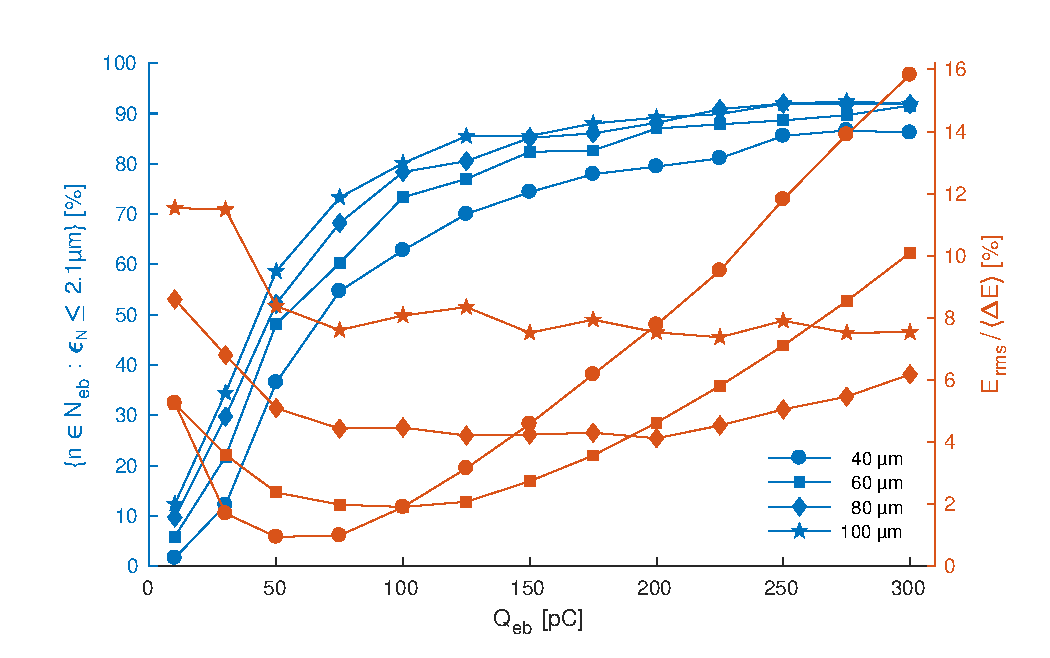
\includegraphics[width=\linewidth,trim={2mm 0mm 2mm 0mm},clip]{figures/beamQuality}
    \caption{\label{Fig:BeamQ} Ratio of total beam charge with an emittance growth $\Delta\epsilon \leq 5\%$ as a
        function of initial beam charge (blue), and relative energy spread of the accepted charge (red), after
        $4\unit{m}$ of plasma and with an initial emittance $\epsilon_{N,0}=2\unit{\mu m}$. These are shown for four
        different $\sigma_{z}$ from $40\unit{\mu m}$ to $100\unit{\mu m}$. The detailed studies presented in beam
        loading section corrspond to the square marked lines at $100\unit{pC}$.}
\end{figure}

\begin{figure}[hbt]
    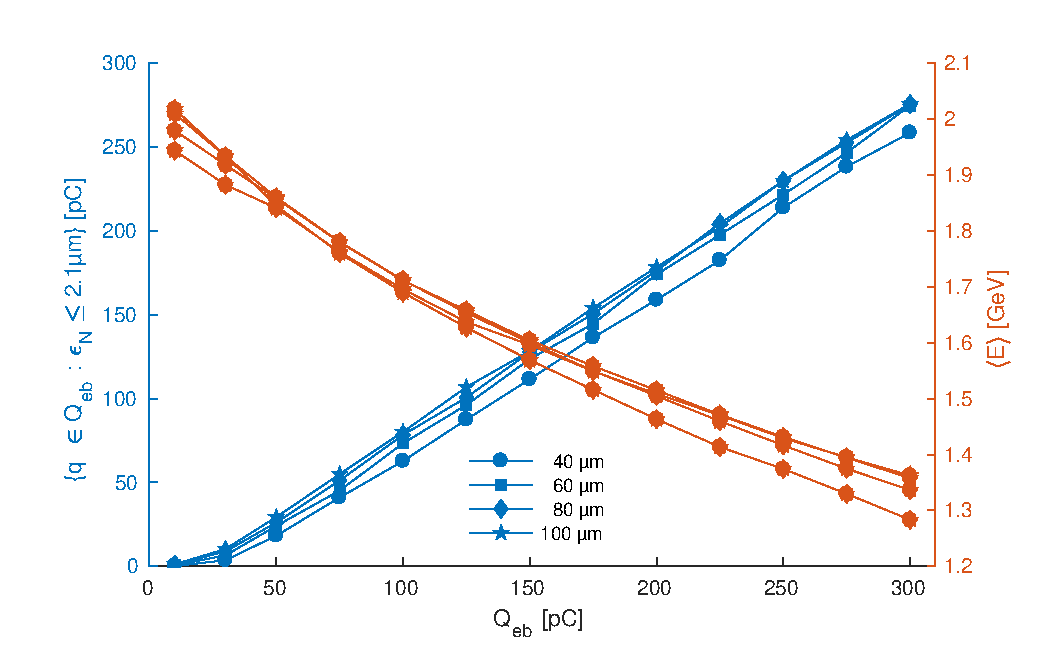
\includegraphics[width=\linewidth,trim={2mm 0mm 2mm 0mm},clip]{figures/beamQualityAbs}
    \caption{\label{Fig:BeamQAbs} Total beam charge with an emittance growth $\Delta\epsilon \leq 5\%$ as a function of
        initial beam charge (blue), and final momentum (red), after $4\unit{m}$ of plasma and with an initial emittance
        $\epsilon_{N,0}=2\unit{\mu m}$.}
\end{figure}

\begin{figure}[hbt]
    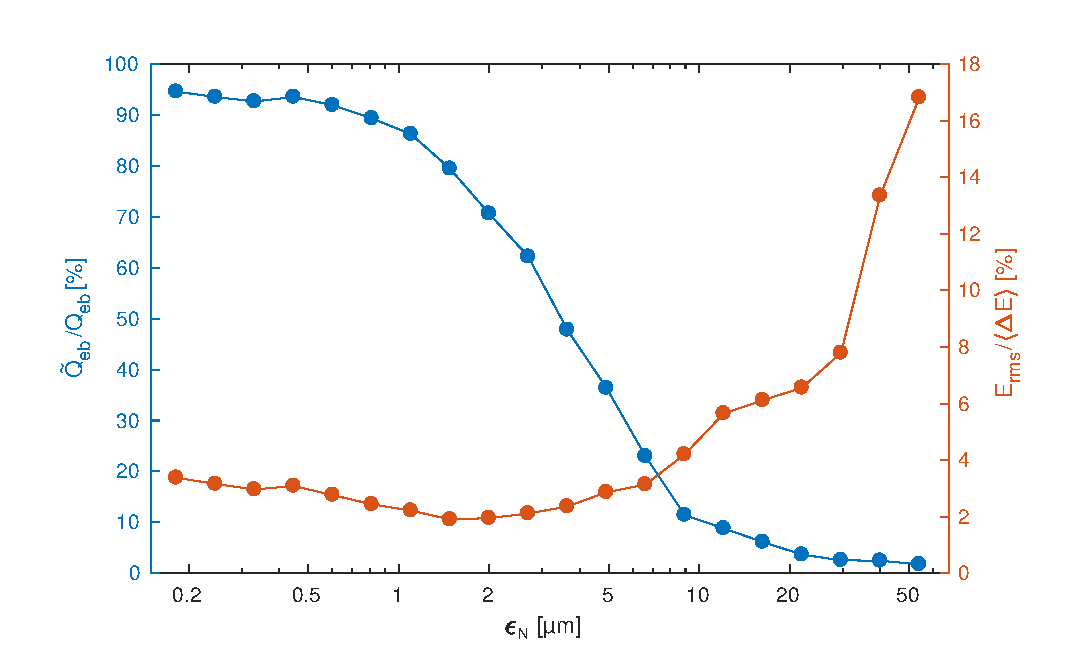
\includegraphics[width=\linewidth,trim={2mm 0mm 2mm 0mm},clip]{figures/beamQualityEmittance}
    \caption{\label{Fig:BeamQEmit} Ratio of total beam charge with an emittance growth $\Delta\epsilon \leq 5\%$ as a
        function of initial emittance (blue), and relative energy spread of the accepted charge (red), after $4\unit{m}$
        of plasma.}
\end{figure}

% ******************************************************************************************************************** %
\section{Parameter Optimisation}\label{S:PO}
%~ Sec N+1: Parameter optimization, or, parameter scaling [in this section we describe how to optimize the electron
%~ beam, and preferably some scalings]
%~ - how to select electron beam parameters:
%~ - longitudinal parameters bunch length and current (simulations results to show: overloaded/underloaded cases)
%~ - transverse parameters of electron emittance / matching [too large, outside bubble.  Do we see increased head
%~   erosion -> faster decay]?  (simulations results to show: evolution of high emittance vs low emittance cases)
%~ (- plasma density?)
% ******************************************************************************************************************** %

The beam loading and blow out properties of the electron beam depends on a large number of parameters, including the
longitudinal profile, the transverse profile as well as the relative phasing of the proton and the electron beams.

%~ We here study parameter optimization relevant for AWAKE Run 2, in order to understand the ideal injection parameters.
For AWAKE Run 2 we desire to maximize the energy gain, minimize the energy spread, maximize the charge to be
accelerated, and minimize the emittance growth. In addition, the bunch length should be such that it is possible to
generate and transport by a compact electron injector \cite{adli:2016}. These are contradictory constraints. We
investigate the interdependence of these parameters in our simulation by varying the electron bunch length, its charge,
and initial emittance. The results were quantified in terms of how much of the initial charge retained its initial
emittance within a $5\%$ margin. For these parameter scans we used a transverse grid cell size of $2.34\unit{\mu m}$,
and let the beams proagate through $4\unit{m}$ of plasma.
%~ We quantify the resulting emittance growth, energy spread and and energy gain. The desired injection parameters will
%~ depend on the application.

Figures \ref{Fig:BeamQ} and \ref{Fig:BeamQAbs} show the dependence on bunch length and bunch charge for an initial beam
emittance of $2\unit{\mu m}$. We ran the scan with beam charges from $10\unit{pC}$ to $300\unit{pC}$ and with length
$\sigma_{z}$ from $40\unit{\mu m}$ to $100\unit{\mu m}$. As can be seen from figure \ref{Fig:BeamQ}, both the
$40\unit{\mu m}$ and the $60\unit{\mu m}$ beam has a well defined minimum energy spread with a beam charge
$\approx 50\unit{pC}$ and $\approx 100\unit{pC}$ respectively. Lower beam charges tend to underload the electric field,
while higher beam charges tend to overload it. It is also clear that longer beams with respect to the accelerating phase
of the field, $\approx\lambda_{pe}/4$, will not optimally load the, thus producing a larger spread in energy.

Figure \ref{Fig:BeamQEmit} shows how the growth in emittance and energy spread varies with initial electron beam
emittance. The smaller the initial emittance is, the better the emittance is preserved. There are two effects that lead
to growth for high emittance beams; the transverse beam size may increase beyond the size of the bubble, or the beam
density may be reduced so much that the plasma electrons are no longer fully evacuated from the ion column. Emittance
values higher than a few micrometres lead to a significant increase in both emittance and energy spread. In these
simulations the focusing of the beam to the plasma remains matched for each emittance value.

% ******************************************************************************************************************** %
\section{Conclusion}\label{S:C}
% ******************************************************************************************************************** %

We have studied a new plasma wakefield acceleration regime; acceleration of a strongly loaded electron beam in a quasi-
linear proton driven wake. When optimally loaded, the electron beam creates its own ion bubble, yielding emittance
preservation for a large parts of the electron beam.

These result indicates that emittance preservation for an on-axis injected electron beam, properly optimized, is
feasible. Parameter studies indicate that up to a few $100\unit{pC}$ might be accelerated, for bunches of length
$40-60\unit{\mu m}$. Such an electron bunch may be generated by a standard S-band RF gun.

As this study assumes a wake driven by a single, short proton beam, the studies for interesting cases for AWAKE should
be repeated by a full simulation of a self-modulated proton beam.

\section{Acknowledgements}\label{Ack}
% ******************************************************************************************************************** %

The simulations for this study have been run using the open source version of QuickPIC released in early 2017 and owned
by UCLA.

These numerical simulations have been made possible through access to the Abel computing cluster in Oslo, Norway. Abel
is maintained by UNINETT Sigma2 AS and financed by the Research Council of Norway, the University of Bergen, the
University of Oslo, the University of Tromsø and the Norwegian University of Science and Technology. Project code:
nn9303k. Some of the simulations were also run on the student-maintained computing cluster ``Smaug'' at the University
of Oslo, Department of Physics.

The authors would also like to thank the OSIRIS Consortium for providing access to the OSIRIS framework. OSIRIS was used
extensively for simulations leading to the work presented in this paper.

% ******************************************************************************************************************** %
\bibliography{Bibliography}
\end{document}
% ******************************************************************************************************************** %
